Conforme mencionado no capítulo \ref{chap:mati}, o desenvolvimento deste trabalho foi dividido em quatro etapas. A primeira etapa envolveu o estudo dos DPDs e dos métodos de modelagem associados. Na segunda etapa, essa modelagem foi implementada em software utilizando a linguagem Python. A terceira etapa consistiu na implementação do modelo de DPD selecionado em hardware, empregando a linguagem VHDL. Por fim, na quarta etapa, foi realizado a síntese lógica para o design do circuito integrado. Este capítulo apresenta os resultados obtidos ao longo do desenvolvimento do projeto.

\section{Modelagem do PA}

Para fazer a modelagem em software foi utilizada a linguagem de programação Python. Para isso, separou-se os dados citados na seção \ref{sec:implsoft} do capítulo \ref{chap:mati}, em dados de extração e dados de validação, os quais são utilizados para extração dos coeficientes do modelo do MP e validação do modelo encontrado, respectivamente. Para fazer a validação do modelo utilizou-se a métrica do NMSE, que consiste em calcular o erro médio quadrado do valor medido pelo VSA para o valor calculado pelo modelo. Portanto, quanto menor o NMSE mais fiel é o modelo do PA. Nesta etapa obteve-se um NMSE de -23.57 dB, para cálculos em vírgula flutuante, onde o resultado está presente no gráfico da figura \ref{fig:modelopafloat}.

\begin{figure}[ht!]
    \centering
    \captionsetup{justification=centering}
    \caption*{Fonte: Autor}
    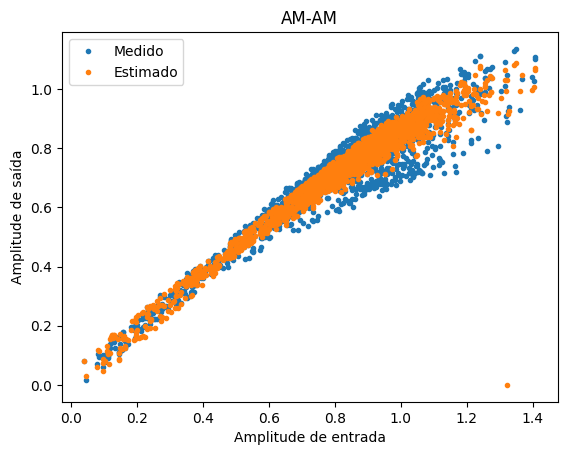
\includegraphics[width=\figsize]{modeloPAfloat.png}
    \caption{Modelo do PA em vírgula flutuante}
    \label{fig:modelopafloat}
\end{figure}

\section{Apuração dos números de bits e resolução do sinal} 

Após concluída a modelagem matemática, foi feita a modelagem do DPD para então ser feito o levantamento da quantidade de bits necessários para a implementação do DPD em hardware minimizando os erros de quantização. 
Para isso foi necessário refazer a extração dos coeficientes, mas desta vez com os dados normalizados para valores de 0 a $2^{bits}$.  
O resultado desse levantamento está presente no gráfico na figura \ref{fig:bits}.

\begin{figure}[ht!]
    \centering
    \captionsetup{justification=centering}
    \caption*{Fonte: Autor}
    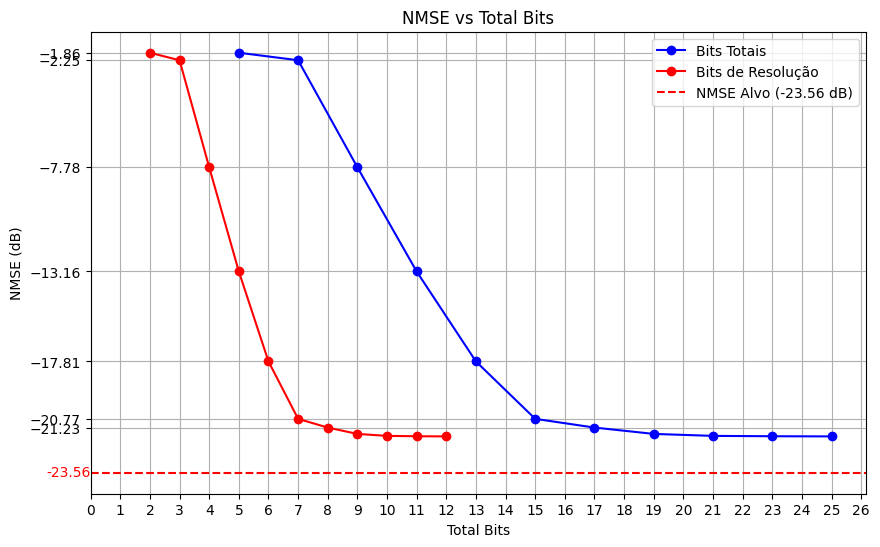
\includegraphics[width=\figsize]{bits.png}
    \caption{Gráfico Número de bits x NMSE}
    \label{fig:bits}
\end{figure}

Neste gráfico observa-se duas curvas, a curva em azul apresenta a quantidade total de bits total contando com os bits de overflow necessárias para as operações de multiplicação, enquanto a curva em vermelho representa a quantidade de bits de resolução do sinal. Analisando este gráfico observou-se que não existem ganhos significativos no erro a partir de 7 bits, portanto foi feita a modelagem do PA utilizando uma resolução de 8 bits o resultado alcançado está ilustrado pela figura \ref{fig:modelopa}.

\begin{figure}[ht!]
    \centering
    \captionsetup{justification=centering}
    \caption*{Fonte: Autor}
    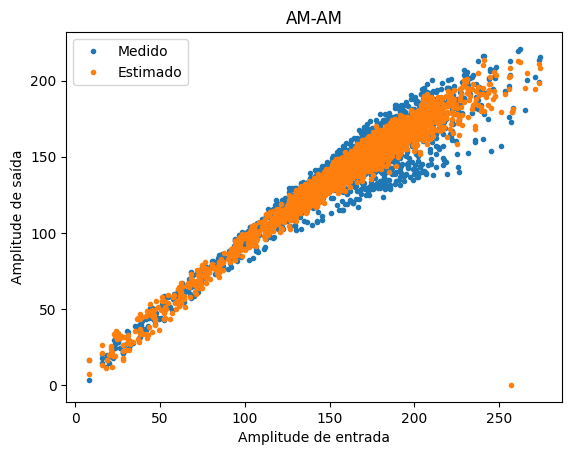
\includegraphics[width=\figsize]{modeloPA.png}
    \caption{Modelo do PA em vírgula fixa}
    \label{fig:modelopa}
\end{figure}

\section{Modelagem do DPD}
A partir dos resultados obtidos foi possível fazer a modelagem do DPD, para isso foi feito o mesmo processo de modelagem do PA, porém para alcançar a característica de transferência inversa PA foi invertido a ordem dos dados de entrada e saída para extração dos coeficientes do DPD. O resultado desta modelagem está ilustrado pela figura \ref{fig:modelodpd} a seguir.

\begin{figure}[H]
    \centering
    \captionsetup{justification=centering}
    \caption*{Fonte: Autor}
    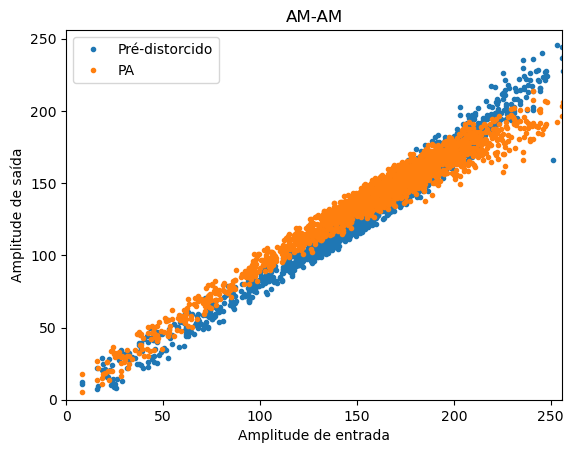
\includegraphics[width=\figsize]{modelodpd.png}
    \caption{Modelo do DPD em vírgula fixa}
    \label{fig:modelodpd}
\end{figure}

\section{Implementação em FPGA}
Em seguida foi feito o código em VHDL para a implementação em FPGA, nessa implementação cada operação aritmética é feita de maneira síncrona, e o fluxo dos cálculos desse processo esta sendo ilustrado pelo diagrama da figura \ref{fig:fluxocal} a seguir.

\begin{figure}[ht!]
	\centering
	\captionsetup{justification=centering}
	\caption*{Fonte: Autor}
	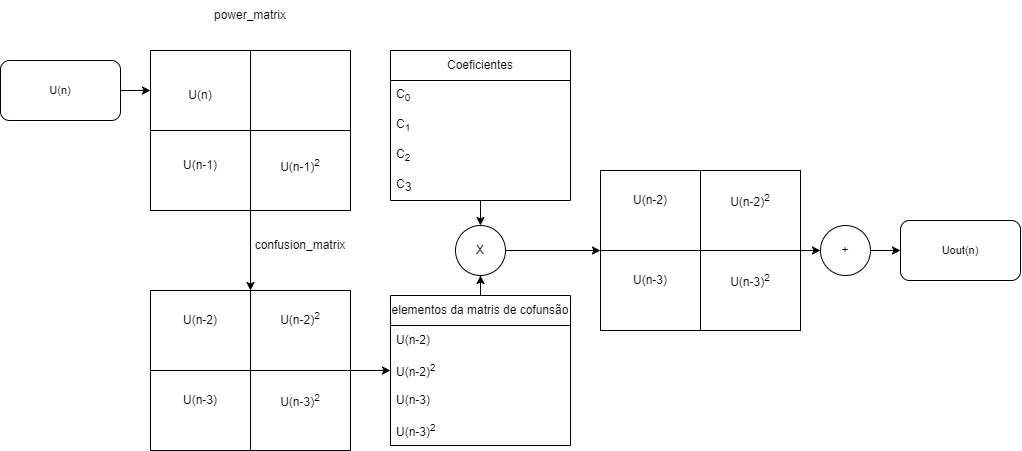
\includegraphics[width=\figsize]{fluxo_de_calculo.png}
	\caption{Fluxo de cálculo FPGA}
	\label{fig:fluxocal}
\end{figure}

No primeiro ciclo de clock é feito o registro do sinal de entrada, para em seguida ele ser elevado ao quadrado N graus do polinômio, para depois esse valor ser adicionado a outro buffer de matriz de extração para para todos os sinais de amostra e por fim ser multiplicado pelos seus respectivos e somado para o sinal de saída.

A figura \ref{fig:simfpga} ilustra o resultado dessa implementação na FPGA Virtex5 XC5VLX50T,utilizando um total de 150 registradores, 692 LUTs e 4 unidades DSP48E, operando a uma frequência de 62,5 MHz.
\begin{figure}[ht!]
	\centering
	\captionsetup{justification=centering}
	\caption*{Fonte: Autor}
	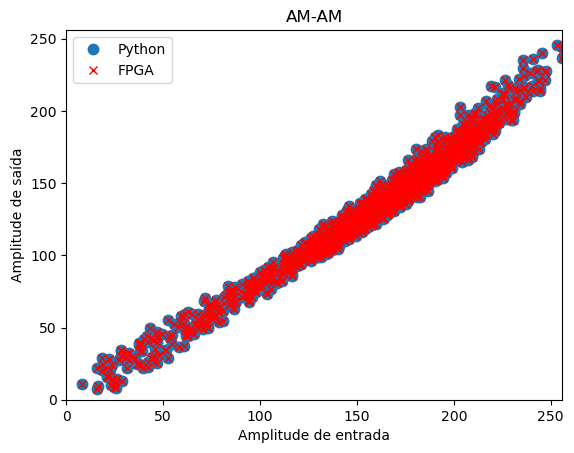
\includegraphics[width=\figsize]{fpgasim.png}
	\caption{Simulação FPGA}
	\label{fig:simfpga}
\end{figure}


\section{Síntese lógica}
Por fim foi feito a síntese lógica do circuito e feita a simulação pós síntese lógica, cujo o resultado esta disponível na Figura \ref{fig:simpost}.

\begin{figure}[ht!]
	\centering
	\captionsetup{justification=centering}
	\caption*{Fonte: Autor}
	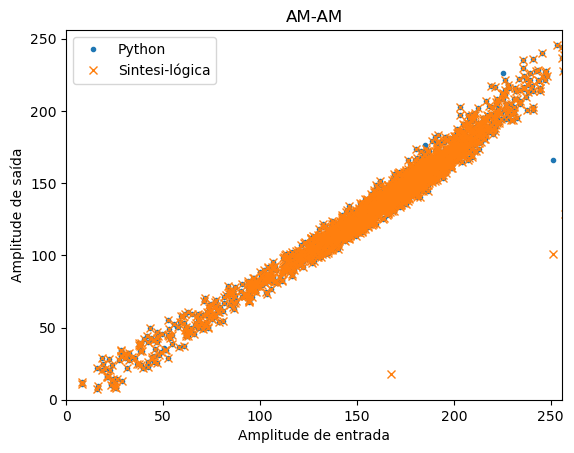
\includegraphics[width=\figsize]{sim_pos_sin.png}
	\caption{Simulação pós síntese}
	\label{fig:simpost}
\end{figure}

Esse circuito resultou em um circuito com 1567 células lógica, com uma area total de 28116 $um^2$ e um consumo de energia de 1.6 mW, atuando a uma taxa de operação de 20 MHz, ou seja, a síntese lógica apresentou um desempenho pior que o apresentado pela FPGA. 